%%%%%%%%%%%%%%%%%%%%%%%%%%%%%%%%%%%%%%%%%%%%%%%%%%%%%%%%%%%%%%%%%%%%%%%%%%%%%%%%
%2345678901234567890123456789012345678901234567890123456789012345678901234567890
%        1         2         3         4         5         6         7         8

\documentclass[letterpaper, 12 pt, conference]{ieeeconf}  % Comment this line out
                                                          % if you need a4paper
%\documentclass[a4paper, 12pt, conference]{ieeeconf}      % Use this line for a4
                                                          % paper

\IEEEoverridecommandlockouts                              % This command is only
                                                          % needed if you want to
                                                          % use the \thanks command
\overrideIEEEmargins
% See the \addtolength command later in the file to balance the column lengths
% on the last page of the document

\usepackage{hyperref}
\usepackage[utf8]{inputenc}
\usepackage{enumerate}
\usepackage{natbib}
\usepackage{graphicx}
\usepackage[spanish]{babel}
\hypersetup{
    colorlinks=true,
    linkcolor=blue,
    filecolor=magenta,      
    urlcolor=cyan,
}

% The following packages can be found on http:\\www.ctan.org
%\usepackage{graphics} % for pdf, bitmapped graphics files
%\usepackage{epsfig} % for postscript graphics files
%\usepackage{mathptmx} % assumes new font selection scheme installed
%\usepackage{times} % assumes new font selection scheme installed
%\usepackage{amsmath} % assumes amsmath package installed
%\usepackage{amssymb}  % assumes amsmath package installed

\title{\LARGE \bf
Práctica 4: 
}

%\author{ \parbox{3 in}{\centering Narshion Ngao*
%         \thanks{*Use the $\backslash$thanks command to put information here}\\
%         Msc. Computer Systems - 2018\\
%         Jomo Kenyatta University of Agriculture \& Technology \\
%       
%}}

\author{Universidad de San Carlos de Guatemala \\% <-this % stops a space
Escuela de Ciencias Físicas y Matemáticas\\
Laboratorio de Circuitos\\
Segundo Semestre 2019
}


\begin{document}



\maketitle
\thispagestyle{empty}
\pagestyle{empty}

\section{Objetivos}
\begin{itemize}
    \item General: estudiar la naturaleza electrónica del diodo.
    \item Específicos:
    \begin{enumerate}
    \item Analizar la precisión de la ecuación de Schokley como modelo del comportamiento de un diodo en directa.
    \item Experimentar los beneficios de las uniones p-n en inversa y directa para fabricación de compuertas lógicas.
\end{enumerate}
\end{itemize}


\section{Materiales}
\begin{itemize}
    \item 2 multímetros.
    \item 1 resistencia 330 ohm 1/4W.
    \item 1 potenciómetro de precisión de 1 Mohm.
    \item 2 diodo rectificadores de silicio.
    \item Alambres para protoboard de cualquier tipo (y pinzas para cortarlo, si es necesario).
    \item 1 fuente.
    \item 1 protoboard.
    \item Opcional: computadora.
\end{itemize}
\pagebreak

\section{Diagramas}

\begin{figure}[h!]
    \centering
    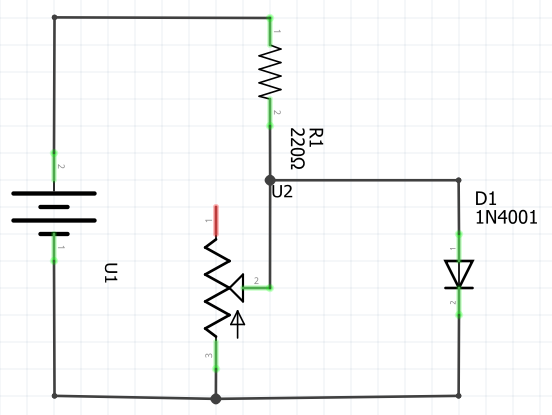
\includegraphics[scale=0.5]{C1.png}
    \caption{Esquema para adquisición de datos.}
\end{figure}

\begin{figure}[h!]
    \centering
    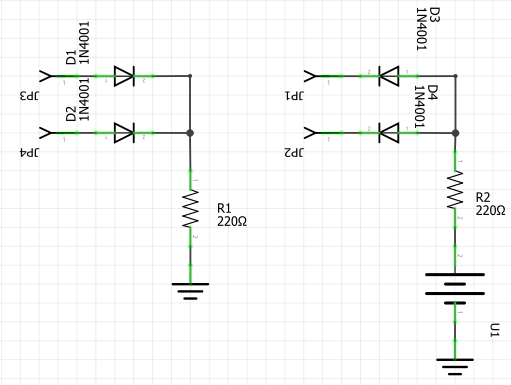
\includegraphics[scale=0.65]{C2.png}
    \caption{Compuertas AND y OR con diodos.}
\end{figure}

\section{Procedimiento y reporte de resultados}
Seguir todos los pasos que a continuación se enlistan respondiendo en una hoja adicional lo que sea requerido de forma ORDENADA y CLARA.

\begin{enumerate}
    \item Armar en protoboard el divisor de voltaje de la Figura 1 para variar la alimentación en el diodo.
\begin{figure}[h!]
    \centering
    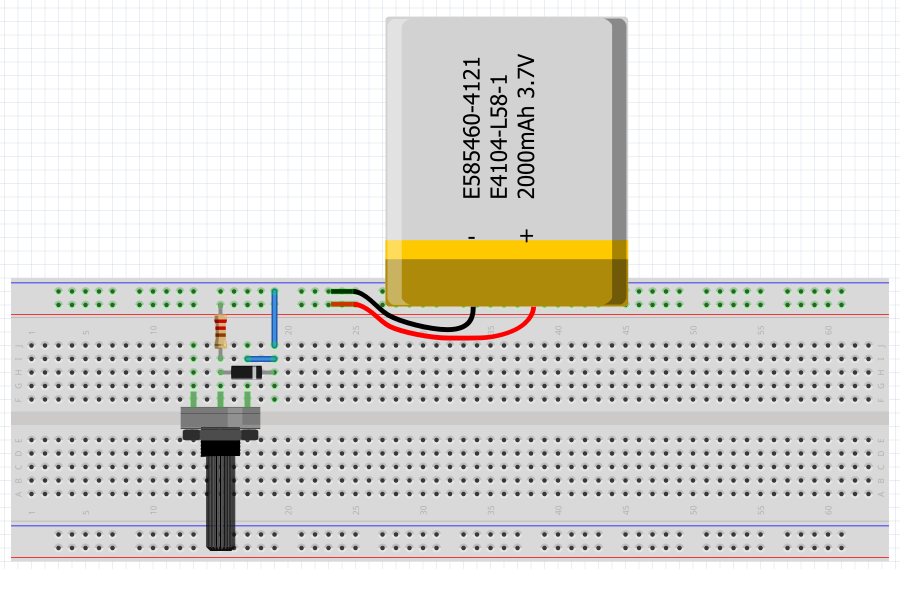
\includegraphics[scale=0.5]{B1.png}
    \caption{Circuito para adquisición de datos.}
\end{figure}
    
    \item Variar con ayuda del potenciómetro la relación de voltaje.
    \item Medir con multímetros la corriente y voltaje del diodo.
    \item Llenar la tabla como se muestra a continuación con QUINCE mediciones:
    
    
    \begin{table}[h!]
    \centering
    \begin{tabular}{|c|l|l|}
    \hline
    \multicolumn{1}{|l|}{\textbf{}} & \textbf{V$\pm\Delta$V} & \textbf{I$\pm\Delta$I} \\ \hline 
    1                               &                  &                  \\ \hline
    2                               &                  &                  \\ \hline
    3                               &                  &                  \\ \hline
    4                               &                  &                  \\ \hline
    \end{tabular}
    \end{table}
    
    \item Con ayuda del software preferido, realizar una gráfica con los puntos obtenidos y encontrar la constante del diodo (n).
    \item Investigar el valor típico de n para el diodo utilizado y comparar.
    \item Armar en protoboard los circuitos de la Figura 2 alimentar con 3.3V o 5V.
    \item Cambiar los valores de entradas según indica la Tabla 2 y medir las salidas para cada circuito. Recordar que un 0 digital indica 0V y 1 digital indica la presencia de un voltaje.
    
\begin{table}[h!]
\centering
\begin{tabular}{|c|c|c|c|}
\hline
\multicolumn{1}{|l|}{\textbf{}} & \multicolumn{1}{l|}{\textbf{In 1}} & \multicolumn{1}{l|}{\textbf{In 2}} & \textbf{Out} \\ \hline
1                               & 0                                  & 0                                  & \textbf{}    \\ \hline
2                               & 1                                  & 0                                  & \textbf{}    \\ \hline
3                               & 0                                  & 1                                  & \textbf{}    \\ \hline
4                               & 1                                  & 1                                  & \textbf{}    \\ \hline
\end{tabular}
\end{table}
    
    \item Según las salidas obtenidas indicar a qué compuerta pertenece cada circuito.
    \item Realizar un reporte completo escrito en LaTex con formato IEEE para presentar resultados de la práctica. Las secciones mínimas requeridas son resumen, objetivos, introducción, marco teórico, diseño experimental, resultados, discusión de resultados y conclusiones.
    
\end{enumerate}
\addtolength{\textheight}{-12cm}   % This command serves to balance the column lengths
                                  % on the last page of the document manually. It shortens
                                  % the textheight of the last page by a suitable amount.
                                  % This command does not take effect until the next page
                                  % so it should come on the page before the last. Make
                                  % sure that you do not shorten the textheight too much.

\end{document}